\documentclass[12pt]{article}
\usepackage{ctex}
\usepackage[english]{babel}
\usepackage{blindtext}
\usepackage{nameref}
\usepackage{fancyhdr}
\usepackage{amsmath,amssymb,amsthm}
\usepackage{graphicx,float}
\usepackage{physics}
\usepackage{pgfplots}
\usepackage[a4paper, total={6in, 9in}]{geometry}

\graphicspath{{../image/}}

\pagestyle{fancy}
\fancyhf{}
\fancyhf[HL]{微分}
\fancyhf[CF]{\thepage}

\newcommand{\innerprod}[2]{\langle{#1},{#2}\rangle}
\newcommand{\id}{\mathtt{id}}

\newtheorem{definition}{定義}
\newtheorem*{theorem}{定理}
\newtheorem*{corollary}{衍理}
\newtheorem*{lemma}{引理}
\newtheorem*{proposition}{設理}
\newtheorem*{remark}{小記}
\newtheorem*{claim}{主張}
\newtheorem*{example}{例子}
\newtheorem*{axiom}{公設}
\renewenvironment*{proof}{\textit{證明.}}{\hfill$\qed$}

\newenvironment*{sol}{\par \textbf{解}.}{\hfill$\blacksquare$}

\begin{document}
    References: Introduction to Real Analysis (Bartle \& Sherbert), Thomas Calculus 12th Edition
    \section*{單元導數定義}

    由牛頓發揚光大的流數法,今時今日變成了以極限定義的導數。

    \begin{definition}[導數定義]
        若$f$在$c$可導,則其導數$f'(c)$為$$f'(c)=\lim_{x\to c}\frac{f(x)-f(c)}{x-c}$$
    \end{definition}

    \begin{definition}[現代導數嚴謹定義]
        $L$為$f$在$c$的導數當:對於任意$\epsilon>0$,若存在$\delta(\epsilon)>0$使得對於$0<|x-c|<\delta(\epsilon)$,$$|\frac{f(x)-f(c)}{x-c}-L|<\epsilon$$
        則寫$f'(c)=L$。
    \end{definition}

    \begin{example}
        $f(x):=x^2$在$c$可微。

        \begin{align*}
            f'(c)&=\lim_{x\to c}\frac{f(x)-f(c)}{x-c}\\
            &=\lim_{x\to c}\frac{x^2-c^2}{x-c}\\
            &=\lim_{x\to c}(x+c)\\
            &=2c
        \end{align*}
    \end{example}

    \begin{theorem}
        若$f:I\to\mathbb{R}$在$c\in I$可微,則$f$在$c\in I$連續。
    \end{theorem}

    \begin{proof}
        導數存在,則\begin{align*}
            \lim_{x\to c}(f(x)-f(c))&=\lim_{x\to c}\frac{f(x)-f(c)}{x-c}\cdot \lim_{x\to c}(x-c)\\
            &=f'(c)\cdot 0\\
            &=0
        \end{align*}
        因此$\displaystyle\lim_{x\to c}f(x)=f(c)$使得$f$在$c\in I$連續。
    \end{proof}

    導數的目的在於處理函數的變化:從算式可見,導數取自$f$的變化除以變量$x$的變化,即可理解爲變化的比例,等於變化比率。簡而言之,導數為函數的斜率。

    \begin{example}[基本導數定則]
        \begin{enumerate}
            \item 常函數的導數:$$\frac{d}{dx}(c)=0$$
            \item 冪函數的導數:$$\frac{d}{dx}(x^n)=nx^{n-1}$$
            \item 自然指數的導數:$$\frac{d}{dx}(e^x)=e^x$$
            \item 自然對數的導數:$$\frac{d}{dx}(\ln|x|)=\dfrac{1}{x}$$
            \item 三角函數的導數:\begin{enumerate}
                \item $$\frac{d}{dx}(\sin{x})=\cos{x}$$
                \item $$\frac{d}{dx}(\cos{x})=-\sin{x}$$
                \item $$\frac{d}{dx}(\tan{x})=\sec^2{x}$$
            \end{enumerate}
        \end{enumerate}
    \end{example}

    \begin{proof}
        留做習題。
    \end{proof}

    \begin{theorem}[導數的性質]
        導數擁有以下性質:\begin{enumerate}
            \item 綫性性:對於可微函數$f,g$,常數$\alpha,\beta$,$(\alpha f+\beta g)'=\alpha f' + \beta g'$。
            \item 乘積法則:對於連續函數$f,g$,$(f\cdot g)'=f'\cdot g + f\cdot g'$。
            \item 除法定則:對於連續函數$f,g$,$(\frac{f}{g})'=\frac{f'\cdot g-f\cdot g'}{g^2}$。
        \end{enumerate}
    \end{theorem}

    \begin{proof}
        \begin{enumerate}
            \item 綫性性:從$f,g$的可微性,可得對任意$\varepsilon>0$,均有$\delta_f,\delta_g>0$使得對於所有$c$,若$x$符合$0<|x-c|<\min\{\delta_f,\delta_g\}$時,$$|\frac{f(x)-f(c)}{x-c}-f'(c)|<\frac{\varepsilon}{2\alpha};|\frac{g(x)-g(c)}{x-c}-g'(c)|<\frac{\varepsilon}{2\beta}$$
            則\begin{align*}
                &|\frac{(\alpha f(x)+\beta g(x))-(\alpha f(c)+\beta g(c))}{x-c}-(\alpha f'(c)+\beta g'(c))|\\
                &<\alpha|\frac{f(x)-f(c)}{x-c}-f'(c)|+\beta|\frac{g(x)-g(c)}{x-c}-g'(c)|\\
                &<\alpha\cdot\frac{\varepsilon}{2\alpha}+\beta\cdot\frac{\varepsilon}{2\beta}\\
                &=\varepsilon
            \end{align*}
            \item 乘積法則:從$f,g$的可微性,可得
            \begin{align*}
                \lim_{x\to c}\frac{f(x)g(x)-f(c)g(c)}{x-c} &= \lim_{x\to c}\frac{f(x)g(x)-f(x)g(c)+f(x)g(c)-f(c)g(c)}{x-c}\\
                &=\lim_{x\to c}(\frac{f(x)-f(c)}{x-c}\cdot g(c)+f(x)\cdot \frac{g(x)-g(c)}{x-c})\\
                &=f'(c)g(c)+f(c)g'(c)
            \end{align*}
            \item 除法定則:留作習題
        \end{enumerate}
    \end{proof}

    \begin{example}
        若$f,g$為可微函數使得$f(c)=1, g(c)=c^2, f'(c)=1$及$g'(c)=2c$,則:\begin{enumerate}
            \item $(2f+3g)'(c)=2f'(c)+3g'(c)=2+6c$。
            \item $(fg)'(c)=f'(c)g(c)+f(c)g'(c)=c^2+2c$。
            \item $(f/g)'(c)=(f'(c)g(c)-f(c)g'(c))/(g(c))^2=c^{-2}-2c^{-3}$。
        \end{enumerate}
    \end{example}

    \begin{corollary}
        導數擁有以下性質:\begin{enumerate}
            \item 綫性性:對於一系列可微函數$\{f_k\}_{k=1}^n$,及一系列常數$\{\alpha_k\}_{k=1}^n$,$\displaystyle(\sum_{k=1}^{n}\alpha_k f_k)'=\sum_{k=1}^{n}(\alpha_k f_k')$。
            \item 乘積法則:對於一系列可微函數$\{f_k\}_{k=1}^n$,$\displaystyle(\prod_{k=1}^{n}f_k)'=\sum_{k=1}^{n}(f_1f_2\cdots f_k'\cdots f_{n-1}f_n)$。
        \end{enumerate}
    \end{corollary}

    \begin{theorem}[鏈鎖律]
        對於複合函數$h:=(g\circ f)$,$$h'=(g'\circ f)\cdot(f')$$
    \end{theorem}

    證明以上定理需引用一下引理:

    \begin{lemma}
        設$f:I\to\mathbb{R}$,$c\in I$。則$f$可微當且僅當存在函數$\varphi$在$I$上定義且於$c$點連續使得對於所有$x\in I$均有$$f(x)-f(c)=\varphi(x)(x-c)$$則寫$\varphi(c)=f'(c)$。
    \end{lemma}

    \begin{proof}[引理]
        若$f'(c)$存在,即$$\varphi(x):=\begin{cases}
            \frac{f(x)-f(c)}{x-c}, & x\neq c\\
            f'(c), & x=c
        \end{cases}$$為連續函數,使得$\varphi(c)=f'(c)$。

        若$\varphi$為連續函數符合$$f(x)-f(c)=\varphi(x)(x-c)$$則$$\varphi(c)=\lim_{x\to c}\varphi(x)=\lim_{x\to c}\frac{f(x)-f(c)}{x-c}=f'(c)$$
    \end{proof}

    \begin{proof}[鏈鎖律]
        對任意$c\in I$,存在$\varphi_c,\phi_c$使得下列成立
        \begin{align*}
            h(x)-h(c)&=g(f(x))-g(f(c))\\
            &=\varphi_c(f(x))(f(x)-f(c))\\
            &=\varphi_c(f(x))\cdot \phi_c(x)(x-c)
        \end{align*}
        因此,$h'(c)=\varphi_c(f(c))\cdot \phi_c(c)=g'(f(c))\cdot f'(c)$。
    \end{proof}

    \begin{example}
        設$h(x):=\sin{e^x}$,則\begin{align*}
            h'(c)&=(\sin)'(e^x)\cdot (e^x)'\\
            &=e^x\cos{e^x}
        \end{align*}
    \end{example}

    \begin{theorem}[逆函數]
        對於逆函數$g:=f^{-1}$,$$g'=\frac{1}{f'\circ g}$$
    \end{theorem}

    \begin{proof}
        設$g(x)=f^{-1}(x)$,則$(f\circ g)(x)=x$。利用鏈鎖律,可得\begin{align*}
            (f'\circ g)(x)\cdot g'(x)&=1\\
            g'(x)&=\frac{1}{(f'\circ g)(x)}
        \end{align*}
    \end{proof}

    \begin{example}
        已知$\ln(x)$為$e^x$的逆函數,則\begin{align*}
            (\ln(x))'&=\frac{1}{e^{\ln(x)}}\\
            &=\frac{1}{x}
        \end{align*}
    \end{example}

    導數可視爲函數於任意點的斜率,換言之,利用直綫方程的點斜式,可得出函數$f$於任意點$(x_0,f(x_0))$上的切綫方程為$$y-f(x_0)=f'(x_0)(x-x_0)$$

    \begin{definition}[高維導數]
        若$f$可微,則$f'$為$f$的第一導數;若$f'$可微,則$f''$為$f$的第二導數,並記$$f''(x)=\dfrac{d}{dx}(f'(x))=\dfrac{d^2}{dx^2}(f(x))$$如此類推,我們稱$f^{(n)}(x)$為$f$的第$n$導數,記$$f^{(n)}(x)=\dfrac{d^n}{dx^n}(f(x))$$
    \end{definition}

    \section*{均值定理}

    均值定理為數學分析其中一個重要工具,亦是導數的重要應用結果。其含義在於將導數與函數值作連接,將切綫普及化。

    \begin{theorem}[極值定理]
        設$c\in I$使得$f:I\to \mathbb{R}$有極值於$c$。若$f$可微,則$f'(c)=0$。
    \end{theorem}

    \begin{proof}
        先證明$f(c)$為極大值的情況:若$f'(c)>0$,則存在$c$的鄰域$V\subseteq I$使得對於$x\in V$,$$\frac{f(x)-f(c)}{x-c}>0$$因此,若$x\in V$同時$x>c$,則$$f(x)-f(c)=(x-c)\cdot\frac{f(x)-f(c)}{x-c}>0$$此則違反$f(c)$為極大值的假設,$f'(c)\not > 0$。

        同理,證明$f'(c)\not < 0$可運用相似做法,因此$f'(c)=0$。
    \end{proof}

    \begin{corollary}
        設$f:I\to\mathbb{R}$為連續函數,並設$f$在$c\in I$有極值。則$f'(c)$不存在或$f'(c)=0$。
    \end{corollary}

    \begin{remark}
        $f(x):=|x|$可作衍理的例證:$f$在$0\in I:=[-1,1]$上存在極小值,但$f'(0)$並不存在。
    \end{remark}

    \begin{theorem}[羅爾定理]
        設$f$在閉合區間$[a,b]$上連續,且可微於開放區間$(a,b)$,使得$f(a)=f(b)=0$。則存在至少一個$c\in(a,b)$使得$f'(c)=0$。
    \end{theorem}

    \begin{theorem}[基本均值定理]
        設$f$在閉合區間$[a,b]$上連續,且可微於開放區間$(a,b)$,則存在至少一個$c\in(a,b)$使得$$f(b)-f(a)=f'(c)(b-a)$$
    \end{theorem}

    \begin{proof}
        設$$\varphi(x):=f(x)-f(a)-\frac{f(b)-f(a)}{b-a}(x-a)$$可見$\varphi$在閉合區間$[a,b]$上連續,且可微於開放區間$(a,b)$,而且$\varphi(b)=\varphi(a)=0$。則可利用羅爾定理引存在$c\in(a,b)$使得$$0=\varphi'(c)=f'(c)-\frac{f(b)-f(a)}{b-a}$$通過簡單移項,便得$$f(b)-f(a)=f'(c)(b-a)$$
    \end{proof}

    逆微分的基本原理,以及第一導數測試,都是從均值定理發展的一些應用。

    \begin{theorem}
        設$f$在閉合區間$I:=[a,b]$上連續,且可微於開放區間$(a,b)$,且$f'(x)=0$對所有$x\in(a,b)$,則$f$為$I$上的常函數。
    \end{theorem}

    \begin{proof}
        利用均值定理,存在至少一個$c\in(a,b)$使得$f(b)-f(a)=f'(c)(b-a)=0$,則$f(a)=f(b)$;並對於所有$x\in(a,b)$,均有$c\in(x,a)$使得$f(x)-f(a)=f'(c)(x-a)=0$。則$f(x)=f(a)$對所有$x\in[a,b]$成立。
    \end{proof}

    \begin{corollary}
        設$f,g$在閉合區間$I:=[a,b]$上連續,且均可微於開放區間$(a,b)$,且$f'(x)=g'(x)$對所有$x\in(a,b)$,則$f=g+C$,其中$C$為常數。
    \end{corollary}

    \begin{definition}[遞升函數]
        設$f$為連續函數,若對於所有$x_1<x_2$均有$f(x_1)\leq f(x_2)$,則稱$f$為遞升函數。
    \end{definition}

    \begin{definition}[遞降函數]
        設$f$為連續函數,若對於所有$x_1<x_2$均有$f(x_1)\geq f(x_2)$,則稱$f$為遞降函數。
    \end{definition}

    \begin{theorem}
        設$f:I\to\mathbb{R}$為可微函數,則:\begin{enumerate}
            \item $f$為遞升函數當且僅當所有$x\in I$均有$f'(x)\geq 0$;
            \item $f$為遞降函數當且僅當所有$x\in I$均有$f'(x)\leq 0$。
        \end{enumerate}
    \end{theorem}

    \begin{proof}
        證明1:設$f'(x)\geq 0$。若$x_1<x_2$,則根據均值定理存在$c\in(x_1,x_2)$使得$$f(x_2)-f(x_1)=f'(c)(x_2-x_1)\geq 0$$
        
        相對地,若$f$為遞升函數,則$$f'(x)=\lim_{x\to c}\frac{f(x)-f(c)}{x-c}\geq 0$$

        證明2:與證明1相似,留做習題。
    \end{proof}

    \begin{theorem}[第一導數測試]
        設$f$為$I:=[a,b]$上的連續函數,並設$c\in(a,b)$。假定$f$在$(a,c)$及$(b,c)$上可微,則:\begin{enumerate}
            \item 若存在$c$的$\delta$-鄰域$(c-\delta,c+\delta)\subseteq I$使得$\begin{cases}
                f'(x)\geq 0, &c-\delta<x<c;\\
                f'(x)\leq 0, &c<x<c+\delta
            \end{cases}$,則$c$為$f$在$I$上的相對極大值;
            \item 若存在$c$的$\delta$-鄰域$(c-\delta,c+\delta)\cap I\subseteq I$使得$\begin{cases}
                f'(x)\leq 0, &c-\delta<x<c;\\
                f'(x)\geq 0, &c<x<c+\delta
            \end{cases}$,則$c$為$f$在$I$上的相對極小值。
        \end{enumerate}
    \end{theorem}

    \begin{proof}
        對於$c-\delta<x<c$時$f'(x)\geq 0$,則根據均值定理,存在$c_x\in(x,c)$使得$$f(c)-f(x)=f'(c_x)(c-x)\geq 0$$則$f(c)\geq f(x)$;同理,對於$c<x<c+\delta$時$f'(x)\leq 0$,則根據均值定理,存在$c_x\in(c,x)$使得$$f(x)-f(c)=f'(c_x)(x-c)\leq 0$$則$f(c)\geq f(x)$。因此,對於$x\in[a,b]$,$f(c)\geq f(x)$,則$f(c)$為相對極大值。

        2的證明與1相似,留做習題。
    \end{proof}

    \section*{洛必達法則}

    洛必達法則主要用來處理不能正常求得的極限,舉例如$f,g$均爲連續函數,而$\displaystyle\lim_{x\to 0}\frac{f(x)}{g(x)}=\frac{0}{0}$的狀況,我們不能直接求得極限的值,因:若定義$f(x)=\alpha x$及$g(x)=x$,$\alpha\in\mathbb{R}$為任意值,則$$\frac{0}{0}=\lim_{x\to 0}\frac{f(x)}{g(x)}=\lim_{x\to 0}\frac{\alpha x}{x}=\alpha$$但洛必達定理通過求導的方法得到了意想不到的結果。

    從最直覺的判斷,我們可以考慮切綫:因爲$\lim_{x\to 0}f(x)=0$及$\lim_{x\to 0}g(x)=0$,因此根據$f,g$的連續性,$f(0)=0$及$g(0)=0$,對於足夠小的$\delta>0$,$x\in(-\delta,\delta)$,$$\begin{cases}
        f(x)\approx f'(0)x\\ g(x)\approx g'(0)x
    \end{cases}$$因此可想像$$\lim_{x\to 0}\frac{f(x)}{g(x)}=\lim_{x\to 0}\frac{f'(0)x}{g'(0)x}=\frac{f'(0)}{g'(0)}$$

    而最基礎的推導也是基於導數定義:

    \begin{theorem}
        設$f,g$均爲$[a,b]$上的函數使得$f(a)=g(a)=0$,並設$g(x)\neq 0$對於$x\in(a,b)$。若$f,g$在$a$點可微且$g'(a)\neq 0$,則$$\lim_{x\to a^+}\frac{f(x)}{g(x)}=\frac{f'(a)}{g'(a)}$$
    \end{theorem}

    \begin{proof}
        \begin{align*}
            \lim_{x\to a^+}\frac{f(x)}{g(x)}&=\lim_{x\to a^+}\frac{f(x)-f(a)}{g(x)-g(a)}\\
            &=\lim_{x\to a^+}\frac{\frac{f(x)-f(a)}{x-a}}{\frac{g(x)-g(a)}{x-a}}\\
            &=\frac{f'(a)}{g'(a)}
        \end{align*}
    \end{proof}

    \begin{remark}
        需注意的是,以上定理只適用於函數在$a$有導數,若$a=\pm\infty$,則需要更多手段。
    \end{remark}

    \begin{theorem}[柯西均值定理/普適均值定理]
        設$f,g$為$[a,b]$上的連續函數,並在$(a,b)$上可微,且$g'(x)\neq 0$對所有$x\in(a,b)$。則存在$c\in(a,b)$使得$$\frac{f(b)-f(a)}{g(b)-g(a)}=\frac{f'(c)}{g'(c)}$$
    \end{theorem}

    \begin{proof}
        設$$h(x):=f(x)-f(a)-\frac{f(b)-f(a)}{g(b)-g(a)}(g(x)-g(a))$$可見$h$在閉合區間$[a,b]$上連續,且可微於開放區間$(a,b)$,而且$h(b)=h(a)=0$。則可利用羅爾定理引存在$c\in(a,b)$使得$$0=h'(c)=f'(c)-\frac{f(b)-f(a)}{g(b)-g(a)}g'(c)$$通過簡單移項,便得$$\frac{f'(c)}{g'(c)}=\frac{f(b)-f(a)}{g(b)-g(a)}$$
    \end{proof}

    \begin{theorem}[洛必達定理I]
        設$-\infty\leq a< b\leq \infty$並設$f,g$於$(a,b)$可微使得所有$x\in(a,b)$均使得$g'(x)\neq 0$。假定$$\lim_{x\to a^+}f(x)=0=\lim_{x\to a^+}g(x)$$\begin{enumerate}
            \item 若$\displaystyle\lim_{x\to a^+}\frac{f'(x)}{g'(x)}=L\in\mathbb{R}$,則$\displaystyle\lim_{x\to a^+}\frac{f(x)}{g(x)}=L$;
            \item 若$\displaystyle\lim_{x\to a^+}\frac{f'(x)}{g'(x)}=L\in\{-\infty,\infty\}$,則$\displaystyle\lim_{x\to a^+}\frac{f(x)}{g(x)}=L$。
        \end{enumerate}
    \end{theorem}

    \begin{proof}
        設$a<\alpha<\beta<b$,根據羅爾定理$g(\alpha)\neq g(\beta)$(爲何?),並根據柯西均值定理,存在$u\in(\alpha,\beta)$使得$$\frac{f(\beta)-f(\alpha)}{g(\beta)-g(\alpha)}=\frac{f'(u)}{g'(u)}$$其中$u\in(\alpha,\beta)$。

        情況1:$L\in\mathbb{R}$,$\varepsilon>0$,存在$c\in(a,b)$使得\begin{align*}
            L+\varepsilon<&\frac{f'(u)}{g'(u)}<L+\varepsilon & u&\in(a,c)\\
            L+\varepsilon<&\frac{f(\beta)-f(\alpha)}{g(\beta)-g(\alpha)}<L+\varepsilon & a<\alpha&<\beta\leq c\\
        \end{align*}
        取$\alpha\to a^+$,可得\begin{align*}
            L+\varepsilon\leq&\frac{f(\beta)}{g(\beta)}\leq L+\varepsilon & \beta&\in(a,c]
        \end{align*}
        因$\varepsilon>0$為任意值,1證畢。

        情況2.1:$L=\infty$,$M>0$,存在$c\in(a,b)$使得\begin{align*}
            \frac{f'(u)}{g'(u)}&>M & u&\in(a,c)\\
            \frac{f(\beta)-f(\alpha)}{g(\beta)-g(\alpha)}&>M & a<\alpha&<\beta\leq c
        \end{align*}
        取$\alpha\to a^+$,可得\begin{align*}
            \frac{f(\beta)}{g(\beta)}&\geq M & \beta&\in(a,c)
        \end{align*}
        因$M>0$為任意值,2.1證畢。

        若$L=-\infty$,證明與2.1類似。
    \end{proof}

    \begin{theorem}[洛必達定理II]
        設$-\infty\leq a< b\leq \infty$並設$f,g$於$(a,b)$可微使得所有$x\in(a,b)$均使得$g'(x)\neq 0$。假定$$\lim_{x\to a^+}f(x)=\pm\infty=\lim_{x\to a^+}g(x)$$\begin{enumerate}
            \item 若$\displaystyle\lim_{x\to a^+}\frac{f'(x)}{g'(x)}=L\in\mathbb{R}$,則$\displaystyle\lim_{x\to a^+}\frac{f(x)}{g(x)}=L$;
            \item 若$\displaystyle\lim_{x\to a^+}\frac{f'(x)}{g'(x)}=L\in\{-\infty,\infty\}$,則$\displaystyle\lim_{x\to a^+}\frac{f(x)}{g(x)}=L$。
        \end{enumerate}
    \end{theorem}

    \section*{泰勒定理}

    回想切綫的出現,可見對於任意可微函數$f$都存在一種估算$$f(x)\approx f(x_0)+f'(x_0)(x-x_0)$$而若需要更精確的估算,考慮若$f$存在二階導數,則$$f(x)\approx f(x_0)+f'(x_0)(x-x_0)+\frac{f''(x_0)}{2}(x-x_0)^2$$同理,若$f$存在三階導數、四階導數,可對$f$進行更精確的估算。如此拓展下去,可得以下定義:

    \begin{definition}[泰勒多項式]
        設$n\in\mathbb{N}$及$I:=[a,b]$,並設$f:I\to\mathbb{R}$使得$f$及其導數$f',f'',\dots,f^{(n)}$均為$(a,b)$上的連續函數,並於$(a,b)$上存在$(n+1)$-階導數$f^{(n+1)}$,則對於$x_0\in I$,設$V(x_0)$為$x_0$的鄰域,可對$x\in V(x_0)$進行以下估算\begin{align*}
            f(x)&\approx f(x_0)+f'(x_0)(x-x_0)+\cdots+\frac{f^{(n+1)}(x_0)}{(n+1)!}(x-x_0)^{n+1}\\
            &=\sum_{k=0}^{n+1}\frac{f^{(k)}(x_0)}{k!}(x-x_0)^k
        \end{align*}
    \end{definition}

    我們記$\displaystyle P_n(x)=\sum_{k=0}^{n+1}\frac{f^{(k)}(x_0)}{k!}(x-x_0)^k$。

    \begin{theorem}[泰勒多項式定理]
        設$n\in\mathbb{N}$及$I:=[a,b]$,並設$f:I\to\mathbb{R}$使得$f$及其導數$f',f'',\dots,f^{(n)}$均為$(a,b)$上的連續函數,並於$(a,b)$上存在$(n+1)$-階導數$f^{(n+1)}$,則對於定點$x_0\in I$,及任意$x\in I$,存在$c$位於$x$與$x_0$之間使得$$f(x)= f(x_0)+f'(x_0)(x-x_0)+\cdots+\frac{f^{(n)}(x_0)}{n!}(x-x_0)^{n}+\frac{f^{(n+1)}(c)}{(n+1)!}(x-x_0)^{n+1}$$
    \end{theorem}

    \begin{proof}
        設$$F(t):=f(x)-\sum_{k=0}^{n}\frac{(x-t)^k}{k!}f^{(k)}(t)$$則\begin{align*}
            F'(t)&=-f'(t)-\sum_{k=1}^{n}\biggl(-\frac{(x-t)^{k-1}}{(k-1)!}f^{(k)}(t)+\frac{(x-t)^k}{k!}f^{(k+1)}(t)\biggr)\\
            &=-f'(t)-(-f'(t)+\frac{(x-t)^{n}}{n!}f^{(n+1)}(t))\\
            &=-\frac{(x-t)^{n}}{n!}f^{(n+1)}(t)
        \end{align*}
        又設$\displaystyle G(t):=F(t)-\biggl(\frac{x-t}{x-x_0}\biggr)^{n+1}F(x_0)$,則見$G(x)=G(x_0)=0$。根據羅爾定理,存在$c$位於$x$和$x_0$之間使得$$0=G'(c)=F'(c)+(n+1)\frac{(x-c)^{n}}{(x-x_0)^{n+1}}F(x_0)$$則\begin{align*}
            F(x_0)&=-\frac{(x-x_0)^{n+1}}{(n+1)(x-c)^n}F'(c)\\
            &=\frac{(x-x_0)^{n+1}}{(n+1)(x-c)^n}\frac{(x-c)^{n}}{n!}f^{(n+1)}(c)\\
            &=\frac{f^{(n+1)}(c)}{(n+1)!}(x-x_0)^{n+1}
        \end{align*}
    \end{proof}

    泰勒定理對相對極值有很大的貢獻。回顧二階導數對極值的影響:

    \begin{theorem}
        設$f:[x_0-\delta,x_0+\delta]\to\mathbb{R}$使得$f$及其導數$f'$均為$(x_0-\delta,x_0+\delta)$上的連續函數,並於$(x_0-\delta,x_0+\delta)$上存在二階導數$f''$使得$f'(x_0)=0$而$f''(x_0)\neq 0$,則\begin{enumerate}
            \item 若$f''(x_0)>0$,$f(x_0)$為相對極小值;
            \item 若$f''(x_0)<0$,$f(x_0)$為相對極大值。
        \end{enumerate}
    \end{theorem}

    \begin{proof}
        證明1:根據泰勒定理,存在$c\in(x_0,x_0+\delta)$使得所有$c'\in(x_0,c)$均有$$f(x)=f(x_0)+\frac{f''(c')}{2}(x-x_0)^2\geq f(x_0)$$同理,存在$d\in(x_0-\delta,x_0)$使得所有$d'\in(d,x_0)$均有$$f(x)=f(x_0)+\frac{f''(d')}{2}(x-x_0)^2\geq f(x_0)$$則$f(x_0)$為$x_0$鄰域上的相對極小值。

        證明2的情況相似,留做習題。
    \end{proof}

    因此利用泰勒定理,可將上述極值的定理拓展至高階導數版本:

    \begin{theorem}
        設$f:[x_0-\delta,x_0+\delta]\to\mathbb{R}$使得$f$及其導數$f',f'',\dots,f^{(n-1)}$均為$(x_0-\delta,x_0+\delta)$上的連續函數,並於$(x_0-\delta,x_0+\delta)$上存在$n$階導數$f^{(n)}$使得$f'(x_0)=f''(x_0)=\cdots=f^{(n-1)}(x_0)=0$而$f^{(n)}(x_0)\neq 0$,則\begin{enumerate}
            \item 若$n$為偶數而$f^{(n)}(x_0)>0$,$f(x_0)$為相對極小值;
            \item 若$n$為偶數而$f^{(n)}(x_0)<0$,$f(x_0)$為相對極大值;
            \item 若$n$為奇數,則$f(x_0)$並非極值。
        \end{enumerate}
    \end{theorem}

    \begin{proof}
        證明留做習題。
    \end{proof}

    另外還有一種導數的應用,在於尋找函數的根。我們以往可以利用分割法進行推演,但效率實在太低;因此牛頓發明了更快捷的做法,我們稱其爲牛頓分割法。

    此方法利用切綫做切入,加速靠近根點。因此,通過數列的創造,可不斷接近根點。考慮$$y-f(x_n)=f'(x_n)(x-x_n)$$代$y=0$可得$x$軸切點,則爲數列的新一項:$$-f(x_n)=f'(x_n)(x_{n+1}-x_n) \implies x_{n+1}=x_n-\frac{f(x_n)}{f'(x_n)}$$

    \begin{theorem}[牛頓分割法]
        設$I:=[a,b]$並設$f:I\to\mathbb{R}$為二階可微函數。假定$f(a)f(b)<0$並存在$m,M>0$使得所有$x\in I$均符合$|f'(x)|\geq m>0$及$|f''(x)|\leq M$。設$K:=M/2m$。則存在$r\in I'\subset I$使得$f(r)=0$,同時有數列$(x_n)$定義爲$$x_{n+1}:=x_n-\frac{f(x_n)}{f'(x_n)}$$使得$\displaystyle\lim_{n\to \infty}x_n=r$,而且$|x_{n+1}-r|<K|x_n-r|^2$。
    \end{theorem}

    \begin{proof}
        留做習題。

        提示:\begin{enumerate}
            \item $f(a)f(b)<0\implies f(a)$和$f(b)$一正一負。根據介值定理得到$r\in(a,b)$使得$f(r)=0$。
            \item 考慮泰勒多項式$$0=f(r)=f(x_n)+f'(x_n)(x_n-r)+\frac{f''(c)}{2}(x_n-r)^2$$其中$x_n\in I$,$c$介乎$x_n$與$r$之間。
            \item 考慮$$x_{n+1}=x_n-\frac{f(x_n)}{f'(x_n)}$$得到$|x_{n+1}-r|<K|x_n-r|^2$。
            \item 設$\delta<1/K$完成極限證明。
        \end{enumerate}
    \end{proof}

    \newpage

    \section*{繪圖}

    繪圖的目的在於一更直觀的方式理解函數的整體運作,因此有數樣東西需要在繪圖前知道:\begin{enumerate}
        \item 軸的切點;
        \item 最高與最低點;
        \item 鞍點;
        \item 漸近綫。
    \end{enumerate}

    \begin{example}
        繪畫$y=\displaystyle\frac{\sin{x}}{x}$的圖像。

        \begin{sol}
            \begin{enumerate}
                \item \begin{enumerate}
                    \item $x$軸切點:令$y=0$,則$\sin{x}=0$。因此,圖像與$x$軸相交於$x=n\pi$,$n\in\mathbb{Z}$。但$x=0$未定義,因此$n\in\mathbb{Z}\setminus\{0\}$。
                    \item $y$軸切點:$x=0$未定義,但$\displaystyle\lim_{x\to 0}\frac{\sin{x}}{x}=1$,因此$y$軸切點虛設於1。
                \end{enumerate}
                \item $y'=\displaystyle\frac{x\cos{x}-\sin{x}}{x^2}$。設$y'=0$則$\tan{x}=x$。欲求$\tan{x}=x$的解可視爲求$\tan{x}-x$的根,又知$\tan{x}$的周期為$(n\pi-\pi/2,n\pi+\pi/2)$,則可運用牛頓法求根。
                
                設$f(x):=\tan{x}-x$,則$f'(x)=\sec^2{x}-1=\tan^2{x}$。利用$$x_{n+1}=x_n-\frac{f(x_n)}{f'(x_n)}=x_n-\frac{\tan{x_n}-x_n}{\tan^2{x_n}}$$可知根的集合為$$\{0,\pm 4.4934, \pm 7.2525, \dots\}$$

                $y''=\displaystyle\frac{(2-x^2)\sin{x}}{x^3}$。則可檢查
                \begin{center}
                    \begin{tabular}{|c|c|c|c|c|c|c|c|}
                        \hline
                        $x$&$\cdots$&$-7.25$&$-4.49$&$0$&$4.49$&$7.25$&$\cdots$\\
                        \hline
                        $y''$&$\cdots$&$-$&$+$&$\lim_{x\to 0}y''<0$&$+$&$-$&$\cdots$\\
                        \hline
                    \end{tabular}
                \end{center}
                \item 沒有鞍點。
                \item $\displaystyle\lim_{x\to\infty}y=0$。
            \end{enumerate}
            \begin{figure}[H]
                \centering
                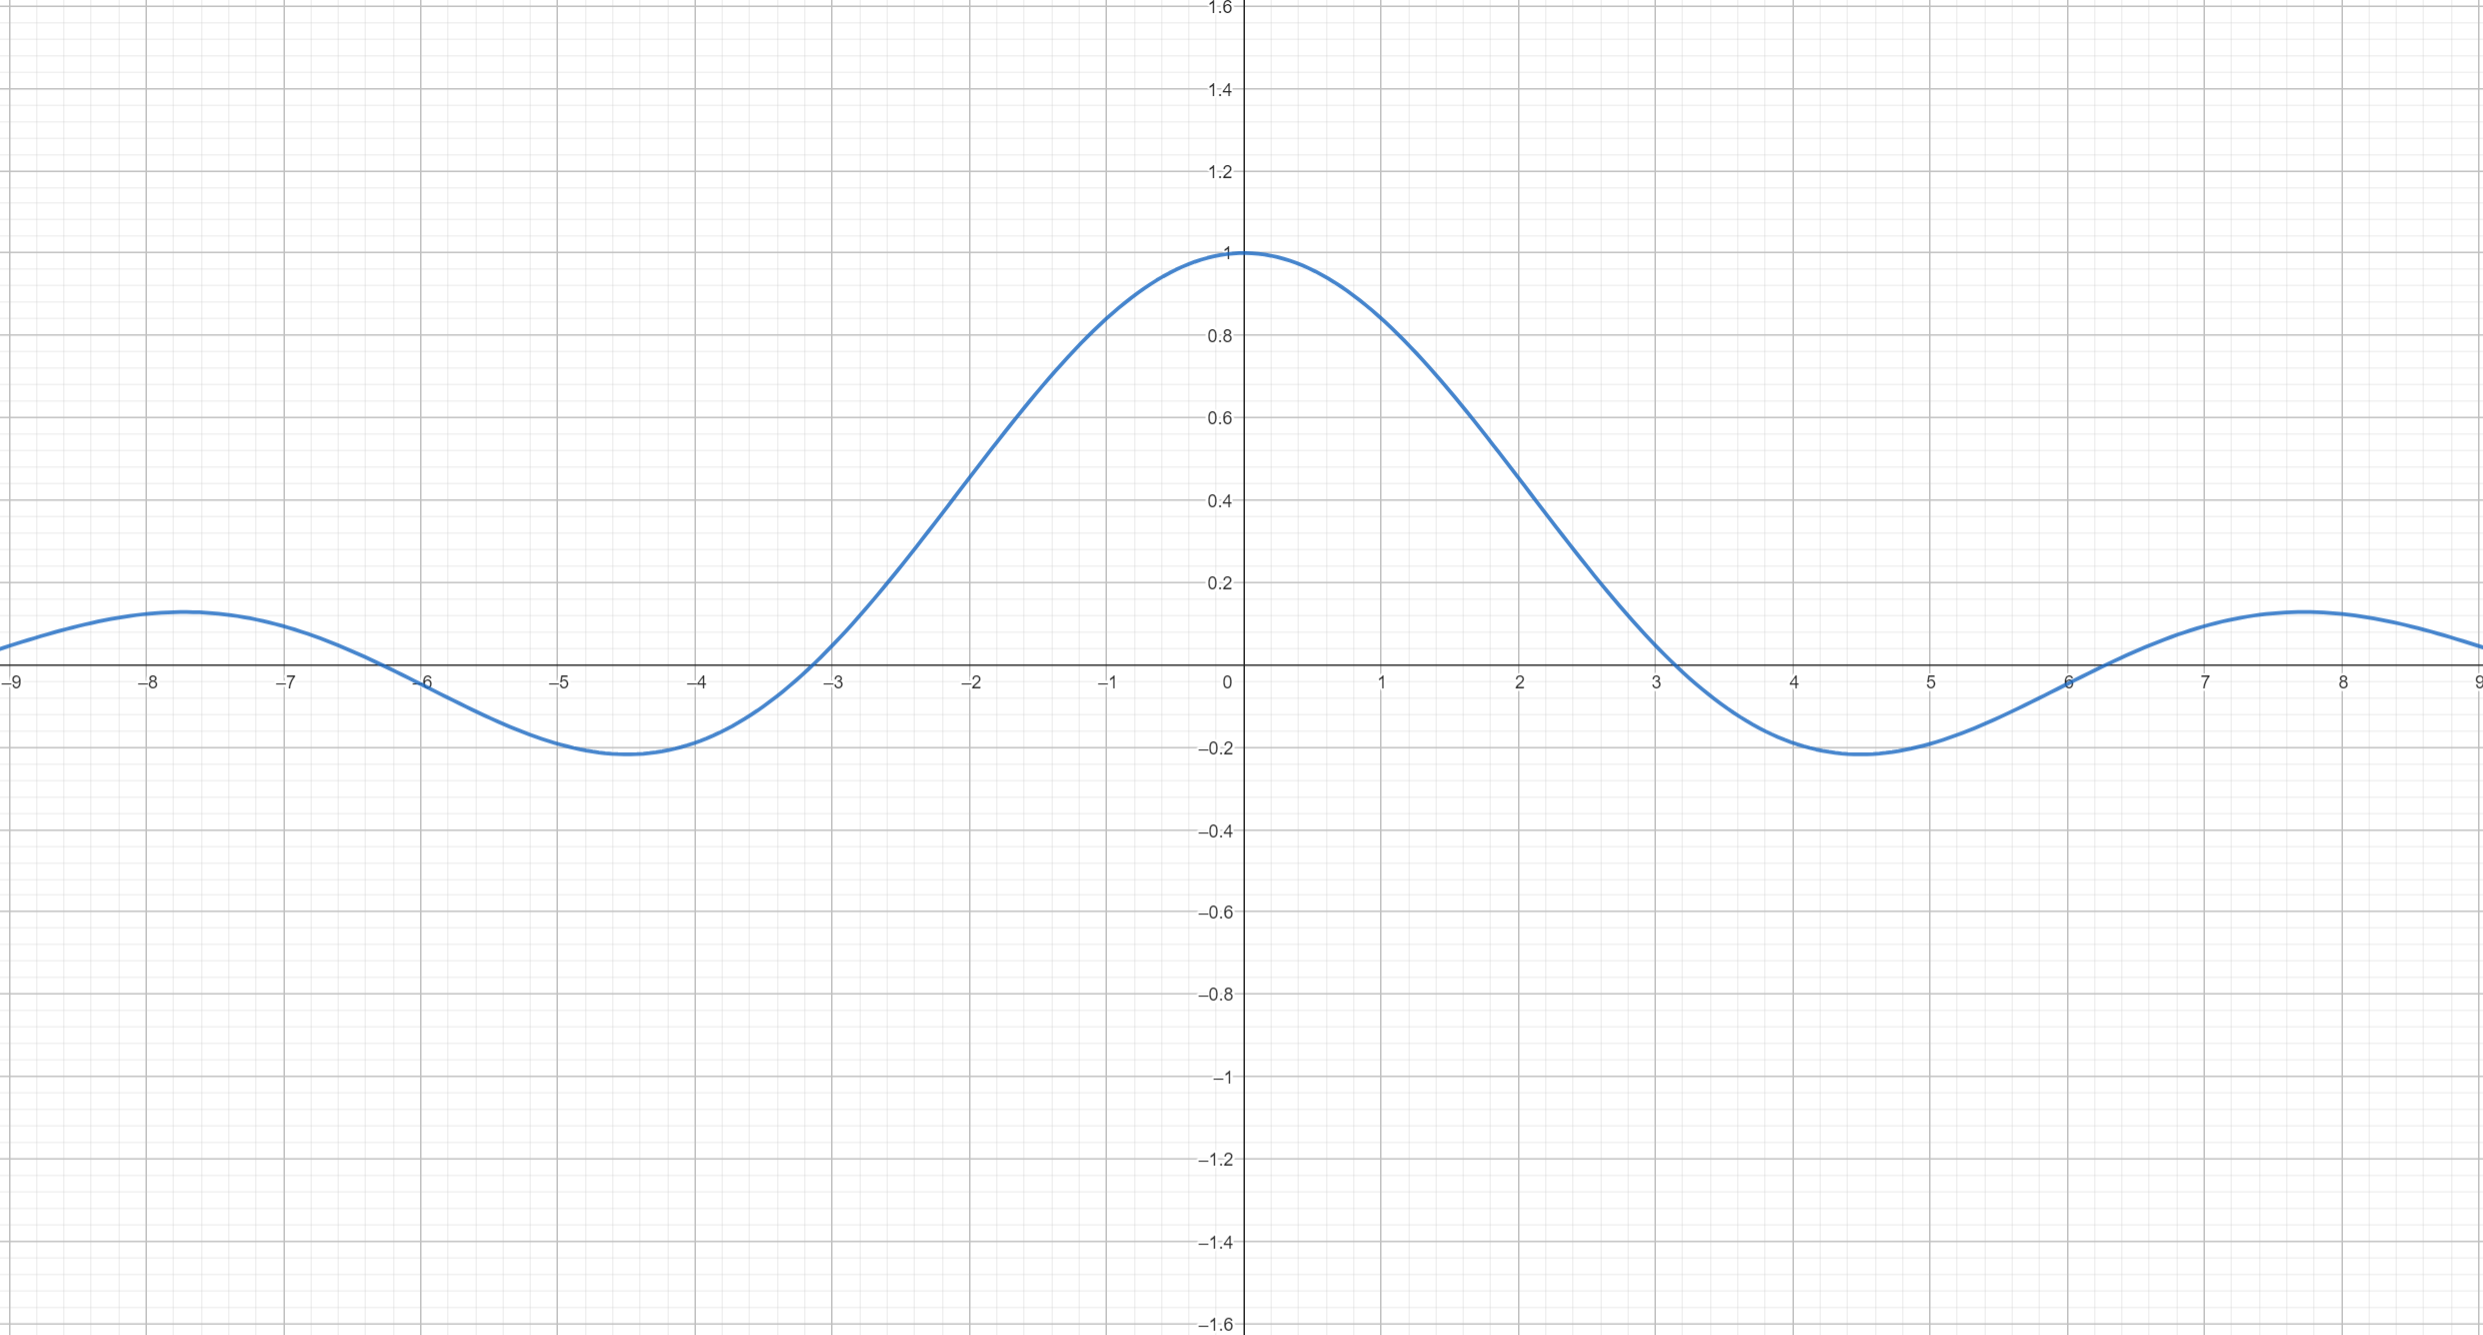
\includegraphics[scale=0.3]{Si(x).png}
            \end{figure}
        \end{sol}
    \end{example}

    \begin{example}
        繪畫$y=\tan{x}-x$的圖像。
        \begin{sol}
            留做習題。
        \end{sol}
    \end{example}
\end{document}